\subsection{Funktionen}
    Das {\annotatorPlugin} soll die Klasse eines Features visualisieren und gleichzeitig
    durch den Benutzer editierbar machen.
    Die Visualisierung besteht aus zwei Teilen und ist in Abbildung
    \ref{image:annotatorPluginViewer} dargestellt.

    % Width vergleichen mit bildern aus einführung
    \begin{figure}[htb]
        \centering
        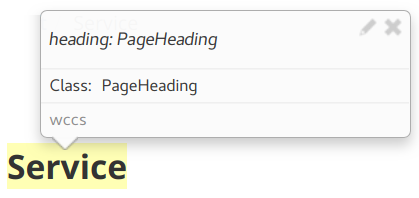
\includegraphics[scale=0.7]{../resources/annotator-plugin/viewer.png}
        \caption{Die Visualisierung einer Klassifikation durch eine Annotation}
        \label{image:annotatorPluginViewer}
    \end{figure}

    Der Name der Klasse ist im Text der Annotation
    enthalten,
    der durch den Nutzer beliebig editiert werden kann.
    Diese Änderung wird zwar nicht
    persistiert,
    ist aber in der Annotation bis zum Neuladen der Webseite sichtbar.
    Aus diesem Grund wird die Klasse nochmals in einem zweiten unveränderlichen Bereich angezeigt,
    welches durch das Plugin ergänzt wird.
    Das Plugin bezieht die Klasse aus dem Feld \texttt{wccs.featureClass}
    der Annotation.
    Wie Abbildung \ref{image:annotatorPluginEditor} zeigt,
    wird dieser zweite Bereich beim Editieren der Annotation zu einer Auswahlliste.

    \begin{figure}[htb]
        \centering
        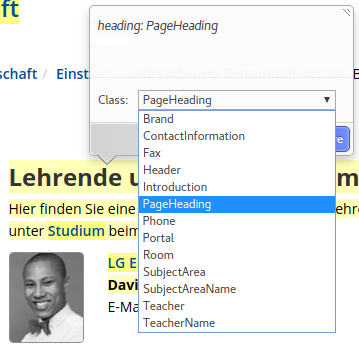
\includegraphics[scale=0.7]{../resources/annotator-plugin/editor.png}
        \caption{Die Korrektur einer Klassifikation durch eine Annotation}
        \label{image:annotatorPluginEditor}
    \end{figure}

    Der Nutzer erhält dadurch die Möglichkeit, die Klasse des Features zu bearbeiten.
    Die Einträge der Auswahlliste sind je nach Art des Features
    Inhalts- oder Referenzklassen, die das {\annotatorPlugin} während seiner
    Initialisierung einmalig vom {\classificationService}
    bezieht.
    Um welche Art von Feature es sich handelt, ermittelt das Plugin anhand des Feldes
    \texttt{wccs.featureKind} der Annotation.
    Beim Speichern wird die ausgewählte Klasse im Feld \texttt{wccs.featureClass} gespeichert.
    Die aktualisierte Annotation wird dann an den {\annotationService} übermittelt,
    welcher die Klasse aus besagtem Feld ausliest und das Feature entsprechend
    aktualisiert.
